\documentclass[12pt]{article}
\usepackage{graphicx}
\usepackage{hyperref}
\usepackage{url}
\usepackage[margin=0.8in]{geometry}
\setlength{\headheight}{0pt}

\title {\textbf{The Sudoku Project}}
\author{Ishika De and Yashvi Donga}
\date{October, 2021}

\begin{document}
    \maketitle
    \section{Objective}
    The goal of this project is to investigate a variety of algorithms
    (backtracking, brute force, stochastic search and Crook’s algorithm) that
    are capable of solving sudoku puzzles, of ranging difficulties, in order to
    learn more about sudoku solving techniques.\\
    We also wanted to use the OpenCV library to read a sudoku from an
    image and solve it.
    \section{Toolchain}
    \begin{itemize}
        \item Languages used: Python, C++, Java.
        \item Libraries used in Python: Numpy, OpenCV and Keras.
    \end{itemize}
    \section{Challenges}
  In the course of this projects we faced a few challenges that helped us learn more about working on a group project and helped us understand our mistakes and improve upon them.\\
   The challenges we faced were as follows:
     \begin{itemize}
		 \item \textbf{Setting unrealistic deadlines}\\
		 While scheduling tasks, we would tend to set overambitious deadlines, that would mess up our schedule and eventually hinder our progress.
		 \item \textbf{Explaining each other's ideas/concepts}\\
		 This project challenged our communication skills. It took us a while to share our ideas and thoughts efficiently. \item \textbf{Failure to implement algorithms}\\
		 We were unable to implement few algorithms like simulated annealing and Crook's algorithm for higher difficulty puzzles. \item \textbf{Dealing with code errors}\\
		 It was difficult for us to move on with failures in code. We would get stuck and would end up spending more than required time on a particular issue.
	 \end{itemize}
%1. Failure to move on
%2. Unrealistic deadlines
%3. Explaining each others ideas
%4. Failure to implement algorithms
    \section{Learnings}
    Through this project we wanted to explore different concepts of programming. In addition to this, we also wanted to learn about neural networks and image processing.\\
    By the end of this project we have learnt to:
     \begin{itemize}
		 \item \textbf{Collaborate using GitLab}\\
		 For this project we chose to use git as our version control tool. It made collaboration easier as we worked on this project remotely. 
		 \item \textbf{Write the same algorithm in different languages}\\
		 We explored the concepts of backtracking and brute force algorithm and implemented these in different languages. We learnt to translate code from one language to another and learnt the pros and cons of each of the languages used. 
		 \item \textbf{Explain our code, thought processes and ideas to each other}\\
		 Initially, communicating our ideas during the ideation of the project was challenging, but, through this project we learnt to explain our codes and ideas to each other efficiently.
		 \item \textbf{Apply the concept of cost function and thermodynamics in simulated annealing}\\
		 Simulated annealing algorithm was an eye opener as it required us to understand concepts of physics - thermodynamics.  The algorithm has an analogy with thermodynamics, specifically with the way that metals cool and anneal.  Simulated annealing calculates optimum of a function instead of the energy of a material.
		 \item \textbf{Process an image to extract digits of a sudoku}\\
		 Image processing was an concept that interested us. We employed the openCV library in python to read a sudoku from an image and subsequently solve it.
		 \item \textbf{Implement neural networks to predict digits of a sudoku from an image}\\
		 To identify the digits from an image we used the MNIST dataset to train the neural network. We learnt how images are fed to a system to capture patterns, in this case, to identify numbers from 1 - 9.
		 \item \textbf{Importance of changeability of code}\\
		 We were able to generate 3 different levels of sudoku just by changing the user input. We generated sudoku puzzles of 3 different difficulties - easy, medium and hard in the three different languages.
	 \end{itemize}
	 
    \section{Results and Conclusion}
    We tested 100 sudoku puzzles in each language for each of the algorithms. The results for the latter are given in the image below.\\
          \begin{figure}[htp]
    		  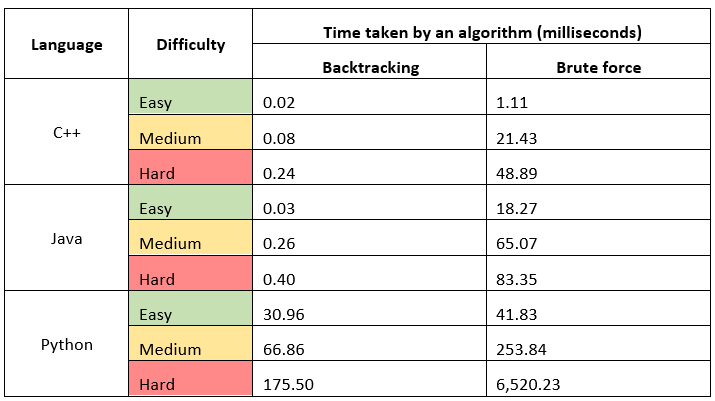
\includegraphics[width=0.8\textwidth]{./week9_img/data.png}
    		  \centering
    		  \caption{Average time taken to solve a sudoku (tested 100 puzzles).}
    		  \centering
		  \end{figure}
	\\As give in the table below, backtracking algorithm was visibly faster than the brute force algorithm in all the languages. While brute-force tries every single possibility, back-tracking follow some path and goes back to previous intersection if it’s a dead-end. This is the reason why backtracking was was much more time-efficient.\\
	\\Considering the languages, C++ took the least amount of time to solve the sudoku and python clearly was the slowest to solve the puzzles, especially puzzles of higher difficulty.\\
	Below is a snapshot of the solved sudoku that was read from an image.
	\begin{figure}[h]
		  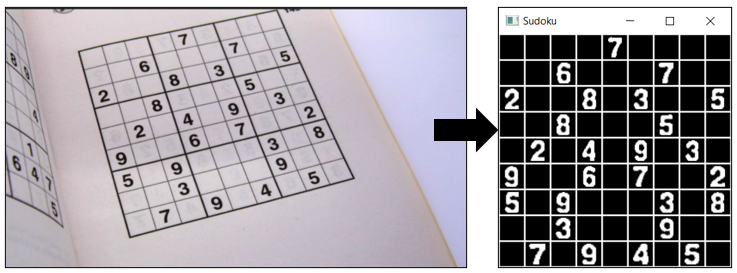
\includegraphics[width=0.7\textwidth]{./week9_img/transformation.png}
		  \centering
		  \caption{Image processing of a sudoku puzzle image.}
		  \centering
		  \end{figure}
	\begin{figure}[!h]
			  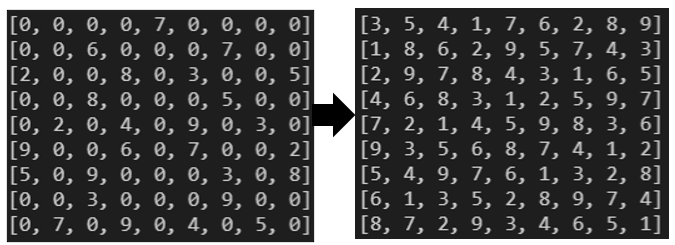
\includegraphics[width=0.7\textwidth]{./week9_img/solve.PNG}
			  \centering
		  \caption{Solved the sudoku from the image}
		  \centering
		  \end{figure}\\
    \section{Code Repository} 
    Our code repository link: \href{https://gitlab.com/yashvidonga29/sudoku-project-we}{\emph{https://gitlab.com/yashvidonga29/sudoku-project-we}}
    \section{References}   
    \begin{itemize}
         \item \sloppy \url{http://people.uncw.edu/tagliarinig/Courses/380/F2015%20papers%20and%20presentations/F2015%20papers%20and%20presentations/Sudoku/Sudoku.pdf}
        \item \sloppy \url{https://towardsdatascience.com/solving-sudoku-with-ai-d6008993c7de}
        \item \sloppy \url{http://zhangroup.aporc.org/images/files/Paper_3485.pdf}
        \item \sloppy \url{https://www.sudokuwiki.org/Brute_Force_vs_Logical_Strategies}
        \item \sloppy \url{https://stacks.stanford.edu/file/druid:my512gb2187/Agarwal_Kamat_Kurian_Smart_Sudoku_Solver.pdf}
        \item \sloppy \url{https://blogs.mathworks.com/deep-learning/2018/11/15/sudoku-solver-image_processing-and-deep-learning}
        \item \sloppy \url{https://www.researchgate.net/publication/264572573_Sudoku_Puzzle_Complexity}
        \item \sloppy \url{https://www.youtube.com/watch?v=FyyVbuLZav8}
        \item \sloppy \url{https://www.adrian.idv.hk/2019-01-30-simanneal/}
        \item \sloppy \url{https://link.springer.com/article/10.1007/s10732-007-9012-8}
        \item \sloppy \url{https://docs.opencv.org/4.5.2/d0/de3/tutorial_py_intro.html}
        \item \sloppy \url{https://www.youtube.com/watch?v=aircAruvnKk}
    \end{itemize}
\end{document}